% 0328(본책 62쪽) — 점 P 에서 원 O 에 그은 두 접선의 접점 A, B, 지름 AC, ∠BAC=18°. 답(∠APB)은 적지 않는다. 스캔 삽화를 TikZ 로 다시 그림.
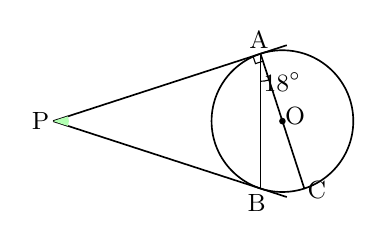
\begin{tikzpicture}[line width=0.6pt]
  \draw (0.000,0.000) circle (0.900);
  \draw (-2.912,0.000) -- (0.055,0.964);
  \draw (-2.912,0.000) -- (0.055,-0.964);
  \draw (-0.278,0.856) -- (-0.278,-0.856);
  \draw (-0.278,0.856) -- (0.278,-0.856);
  \fill (0.000,0.000) circle (1.2pt);
  \draw[line width=0.4pt] (-0.373,0.825) -- (-0.342,0.730) -- (-0.247,0.761);
  \draw[line width=0.4pt] (-0.278,0.506) arc (-90.000:-72.000:0.350);
  \node[font=\small, inner sep=1.5pt] at (0.000,0.500) {$18^\circ$};
  \fill[green!30] (-2.912,0.000) -- (-2.722,-0.062) arc (-18.000:18.000:0.200) -- cycle;
  \node[font=\small, inner sep=1.5pt] at (-3.072,0.000) {P};
  \node[font=\small, inner sep=1.5pt] at (-0.298,1.026) {A};
  \node[font=\small, inner sep=1.5pt] at (-0.328,-1.036) {B};
  \node[font=\small, inner sep=1.5pt] at (0.438,-0.876) {C};
  \node[font=\small, inner sep=1.5pt] at (0.160,0.060) {O};
\end{tikzpicture}
